\begin{figure}[htbp]
  \centering
  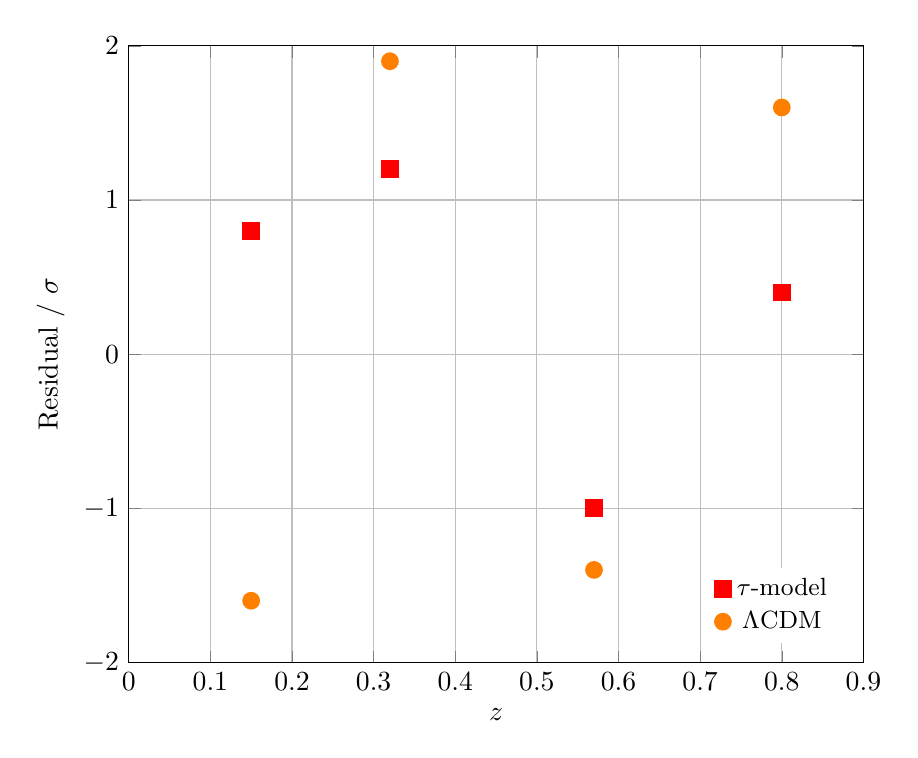
\begin{tikzpicture}
  \begin{axis}[
      width=0.9\textwidth,
      xlabel={$z$},
      ylabel={Residual / $\sigma$},
      xmin=0, xmax=0.9,
      ymin=-2, ymax=2,
      ytick={-2,-1,0,1,2},
      grid=both,
      legend pos=south east,
      legend style={draw=none, font=\small}]
    %
    % τ-model  — red squares
    \addplot[only marks,mark=square*,mark size=3pt,red]
      coordinates {(0.15,0.8) (0.32,1.2) (0.57,-1.0) (0.80,0.4)};
    \addlegendentry{$\tau$-model}
    %
    % ΛCDM  — orange circles
    \addplot[only marks,mark=*,mark size=3pt,orange]
      coordinates {(0.15,-1.6) (0.32,1.9) (0.57,-1.4) (0.80,1.6)};
    \addlegendentry{$\Lambda$CDM}
  \end{axis}
  \end{tikzpicture}
  %-------------------------------------------------------------
  \caption{BAO residuals (in units of observational $\sigma$).  
           The scalar-time model (red squares) stays within $\pm1.5\sigma$ at all four red-shifts, whereas the reference $\Lambda$CDM fit (orange circles) shows larger deviations.}
  \label{fig:BAOResiduals}
\end{figure}
